% Status: DRAFT v4 (readability pass). Numbers: papers/analysis/*.md|json (canonical).
% Build: pdflatex main && bibtex main && pdflatex main && pdflatex main
\documentclass[11pt]{article}
\usepackage[margin=1in]{geometry}
\usepackage{amsmath,amssymb}
\usepackage{graphicx}
\usepackage{booktabs}
\usepackage{xcolor}
\usepackage[colorlinks=true,linkcolor=blue,citecolor=blue,urlcolor=blue]{hyperref}
\usepackage{caption}
\captionsetup{font=small,labelfont=bf}

\title{Certify Before You Optimize:\\ \large A Few Dozen Blind Labels Predict Which LLM Judges Get Gamed}
\author{Anonymous Authors}
\date{Draft v4, August 23, 2026}

\begin{document}
\maketitle

\begin{abstract}
LLM judges now rank models, filter data, and pick the best of $n$ samples, and the standard way to decide whether to trust one is raw agreement with human labels.
That check fails in the worst way: a judge can agree with humans on unoptimized data and still be gamed the moment something optimizes against it.
We introduce a pre-deployment audit: a few dozen blind human labels, graded separately for soundness and for style, reveal whether a judge scores substance or presentation, and yield a verdict of pass, fail, or convict.
We validate the verdicts by running best-of-$n$ selection against every judge and checking who actually gets gamed: the frozen verdicts called the outcome for ten of eleven registered configurations.
The pressure is selection rather than training; the first registered DPO run produced no detectable policy movement (every gain and wedge crossing zero) and was classified post hoc as a manipulation failure, so the predictions went untested, and a stronger rerun carrying a frozen manipulation check is registered and queued.
The audit convicts a deliberately sabotaged frontier judge and a top open reward model, two evaluators that raw agreement cannot tell apart from honest mid-size judges.
The honest pass and the sabotage conviction reproduce significantly on labels from a hypothesis-blind annotator outside the author list; the reward-model conviction reproduces in sign on those labels and is significant on two-rater consensus.
Under pressure, the sabotaged frontier judge inflates its own scoreboard by more than twice the honest judge's inflation while selecting almost as well --- exactly the failure a raw accuracy check cannot see.
The audit costs four to eight annotator-hours of labeling per task and prompt, with one label set serving all thirteen judge configurations here, turning evaluator trust from a post-hoc discovery into a measurement made before deployment.
\end{abstract}


% Main result table, placed here so it renders on page 1 or 2 for skimming reviewers.
\begin{table}[t!]
\centering
\small
\setlength{\tabcolsep}{5pt}
\begin{tabular}{llcccccc}
\toprule
& configuration & verdict & raw $r$ & sound.\ partial & style partial & inflation ($\sigma$) & regret \\
\midrule
blind & 1.5B & convict & $+0.18$ & $-0.00$ & $\mathbf{+0.51}$ & $+0.88$ & $0.448$ \\
ladder & 3B & fail & $+0.24$ & $+0.19$ & $+0.16$ & $+0.44$ & $0.429$ \\
& 7B & fail & $+0.33$ & $+0.32$ & $-0.02$ & $+0.80$ & $0.324$ \\
& 14B & pass$^{*}$ & $+0.37$ & $+0.41$ & $-0.21$ & $+0.63$ & $0.324$ \\
\midrule
referenced & 1.5B & pass & $+0.55$ & $+0.51$ & $+0.10$ & $+0.16$ & $\mathbf{0.010}$ \\
ladder & 3B & pass & $+0.55$ & $+0.53$ & $-0.02$ & $+0.07$ & $0.038$ \\
& 7B & pass & $+0.66$ & $+0.66$ & $-0.12$ & $+0.18$ & $0.019$ \\
& 14B & pass & $+0.70$ & $+0.70$ & $-0.11$ & $+0.05$ & $0.048$ \\
\midrule
frontier & honest & pass & $+0.89$ & $+0.90$ & $-0.22$ & $+0.38$ & $0.117$ \\
(GPT-5.2) & sabotaged & convict & $+0.35$ & $+0.20$ & $\mathbf{+0.59}$ & $+0.85$ & $0.133$ \\
\midrule
sabotaged & 7B & fail & $+0.34$ & $+0.28$ & $+0.17$ & $+0.13$ & $0.400$ \\
ladder & 14B & fail & $+0.45$ & $+0.38$ & $+0.24$ & $+0.61$ & $0.324$ \\
\midrule
reward model & Skywork-8B & convict & $+0.18$ & $-0.01$ & $\mathbf{+0.54}$ & $\mathbf{+1.46}^{\dagger}$ & $0.286$ \\
\bottomrule
\end{tabular}
\caption{\textbf{Main result: a few dozen blind human labels, read through partial correlations, predict which judges get gamed before any optimization runs; raw agreement cannot.
Raw agreement scores the sabotaged frontier judge ($+0.35$) and the honest blind 14B ($+0.37$) nearly identically, while the style partial separates them ($+0.59$ vs.\ $-0.21$) and names the failure mode.}
Each row is one judge configuration on math.
\emph{Verdict}: the frozen audit rule's output (pass, fail, or convict); the verdicts predicted the pressure outcome of ten of the eleven registered configurations (twelve of thirteen counting two late-scored additions; ledger in Table~\ref{tab:ledger}).
\emph{Raw $r$}: plain correlation with human soundness labels (naive validation).
\emph{Sound.\ partial}: correlation with human soundness holding style fixed --- how much substance the judge reads.
\emph{Style partial}: correlation with human style holding soundness fixed --- the property the judge should ignore; significantly positive convicts.
\emph{Inflation}: excess hack gap at best-of-64, in baseline standard deviations --- how far the judge's own scoreboard inflates relative to true quality.
\emph{Regret}: oracle regret --- accuracy left on the table versus best-possible selection.
$n{=}60$ per row except 1.5B blind ($n{=}53$) and 1.5B referenced ($n{=}56$).
Point estimates only; all confidence intervals, and the special-case inference for the 1.5B-blind row, are in Table~\ref{tab:h2h_ci}.
$^{*}$The blind 14B pass is the record's one false pass (Section~\ref{sec:pressure}).
$^{\dagger}$The reward model's inflation uses a candidate-side paraphrase replicate, an analogous but not identical estimand (Section~\ref{sec:limits}).}
\label{tab:h2h}
\end{table}

\section{Introduction}
\label{sec:intro}

Consider a team that wires an LLM judge into best-of-$n$ serving: the model writes 64 candidate solutions per problem and the judge picks the one to keep.
On a spot check the judge agrees with human graders about 90 percent of the time, so the team trusts it.
Under optimization the scoreboard climbs while true quality does not: the pipeline has learned to produce answers the judge likes, not answers that are right, and the judge has been reward-hacked~\cite{gao2022scaling,skalse2022defining}.
The failure was discoverable beforehand, with a few dozen labeled examples, because this judge's scores track writing quality once soundness is held fixed --- and no agreement rate can reveal that.
This paper turns that before-the-fact check into a \emph{certificate}: a cheap audit, run before deployment, whose verdict predicts whether the judge will be gamed.

The workflow the certificate replaces rests on two failing assumptions: that raw human agreement validates a judge, and that nothing better exists before deployment.
Recent work has already shown that benchmark accuracy, the standard static measure of reward-model quality, predicts downstream optimization outcomes poorly~\cite{wen2024rethinking}.
We show that a different static measurement --- what a judge \emph{reads}, not how often it agrees --- does predict them.
That style bias exists in judges and reward models is established at the class level~\cite{wu2023style,rmbench2024}; what the certificate adds is a per-deployment instrument that measures whether a particular judge, on a particular task and prompt, reads substance.

Our contributions:
\begin{itemize}
\item \textbf{A cheap audit with a categorical verdict.} A few dozen blind human labels, graded separately on a target axis (soundness) and an axis the judge should ignore (style), are read through two partial correlations and yield a verdict per judge configuration: pass, fail, or convict (Section~\ref{sec:audit}; Table~\ref{tab:h2h}).
The key verdicts reproduce on a hypothesis-blind non-author rater's labels (Section~\ref{sec:audit}; Table~\ref{tab:robust}).
\item \textbf{Outcome validation under real optimization pressure.} The frozen verdicts predicted the best-of-$n$ outcome for ten of eleven registered configurations; the full registration bookkeeping lives in one prediction ledger (Table~\ref{tab:ledger}), and Section~\ref{sec:pressure} reports the one false pass and the disclosed post-hoc rule revision it triggered.
Because verdicts are collinear with reference presence, the configurations collapse to roughly four verdict classes, so we also report the audit's incremental validity over a reference-presence baseline, which it beats precisely on corrupted evaluators (Section~\ref{sec:audit}; Section~\ref{sec:limits}).
\item \textbf{A diagnosis raw agreement cannot make.} The audit convicts a sabotaged frontier judge and a top open trained reward model that raw agreement scores like honest mid-size judges, and the convicted frontier judge corrupts its scoreboard without measurably corrupting selection --- the failure mode an accuracy check is blind to (Sections~\ref{sec:audit}--\ref{sec:pressure}).
\item \textbf{A generalization path beyond hand labels.} A zero-label perturbation battery and a mechanical-oracle variant of the audit are each validated against the human-label verdicts (Section~\ref{sec:procedure}).
\item \textbf{Design rules for practitioners}, including when a trusted reference helps a judge and when it amplifies gaming (Section~\ref{sec:rules}).
\end{itemize}

The audit can be small because evaluator failure is mechanistic.
Companion work shows that signals which \emph{compare} a solution to reference text fail to grade it, because most of their variance is a property of the reference, while signals that \emph{verify} against something checkable do grade~\cite{companionB}.
A judge sits on one side or the other depending on protocol and scale, and the audit detects which (Figure~\ref{fig:concept}).

Four design choices distinguish the audit from raw-agreement validation.
Humans grade on two separated axes rather than one quality number, because a single number makes loading on the wrong axis unmeasurable in principle; the axes here (soundness, style) are an instantiation chosen for the threat model, not a fixed pair (length, format, and position are probed separately in Section~\ref{sec:rules}).
A deliberately selected subsample --- built where cheap signals disagree, which spreads a soundness axis the random set leaves near ceiling --- supplies power that random data cannot.
The verdict is read from partial correlations, not an agreement rate.
And a sabotaged judge serves as a positive control: evidence the instrument can convict, not merely bless.

We validate by registering predictions and applying pressure: a 7B generator writes 64 candidates per problem, each judge picks its favorite, and two pre-registered quantities separate scoreboard inflation from real accuracy loss (Section~\ref{sec:pressure}).
Failed and convicted judges cluster above correctly certified ones on both quantities; the one false pass sits exactly at the pass threshold (Figure~\ref{fig:h2h}); and a cross-domain extrapolation to code succeeds in ten of eleven eligible configurations, missing exactly where a post-hoc mechanism --- the capability gate --- says the audit itself would not transfer.
That miss yields the operational lesson: certification is a property of a judge, task, and prompt triple, and must be measured where the judge will be used.

\begin{figure}[t]
\centering
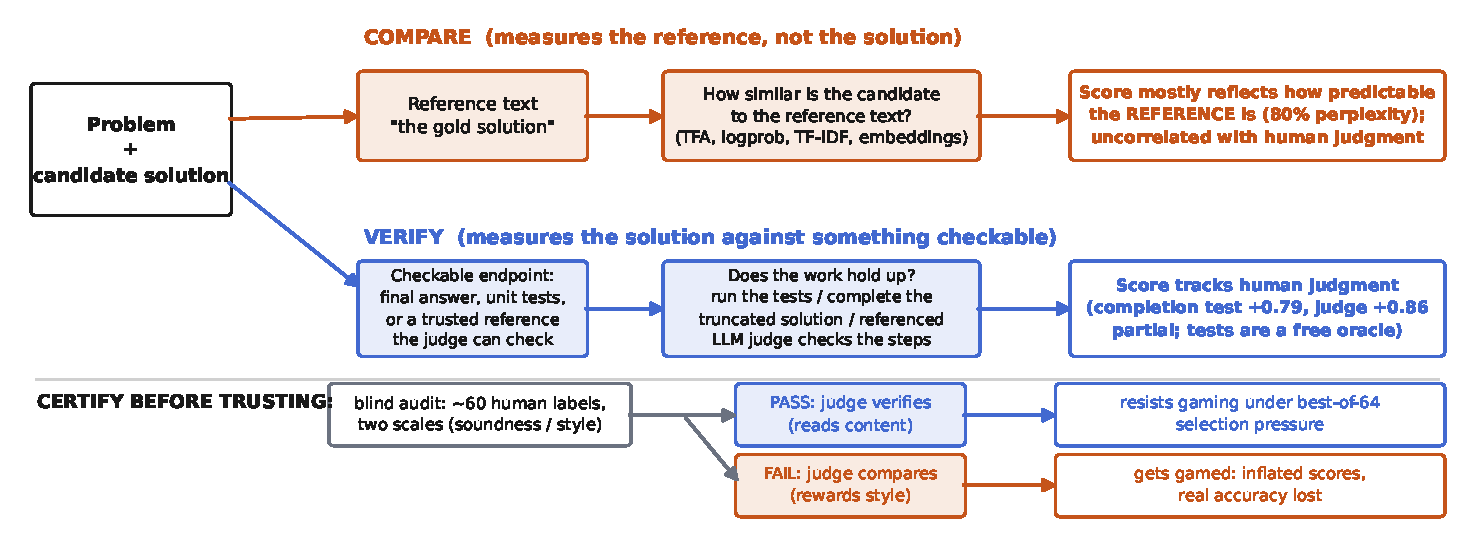
\includegraphics[width=\textwidth]{figures/fig_concept.pdf}
\caption{\textbf{Why a small audit can predict gaming.}
Top and middle: the two evaluator mechanisms; comparison-shaped evaluators reward resemblance to a reference and load on properties like style, while verification-shaped evaluators check the solution against something trusted.
Bottom: the audit pipeline; a blind labeled set read through partial correlations classifies the mechanism, and the verdict predicts behavior under optimization pressure.
\textbf{Takeaway: evaluator failure has one dominant mechanism, so a small instrument aimed at it can predict gaming before any optimization runs.}}
\label{fig:concept}
\end{figure}

\section{Setup}
\label{sec:setup}

\paragraph{Evaluators.}
We audit open-weights judges (Qwen2.5 at 1.5B, 3B, 7B, 14B), each deployed blind and with the gold reference in context, plus GPT-5.2 as the frontier judge and the same frontier model prompted to reward presentation as the sabotaged positive control.
Claude Opus serves as a blind cross-family panel for channel decomposition.
The two sabotaged ladder configurations (7B, 14B) were pressure-tested but never audited, and are excluded from all prediction claims (Appendix~\ref{app:confusion}).
A trained reward model baseline (Skywork-Reward-Llama-3.1-8B) is audited and pressure-tested under predictions registered before its scores were generated.

\paragraph{Human labels.}
The anchor set is a uniformly random sample of \textsc{MATH-500} solutions from seventeen models, graded blind by one annotator on two 0--10 scales with written anchors: \emph{soundness} (is every step valid; ignore the writing) and \emph{style} (is it clear and well-organized; ignore correctness).
Sixty items carry labels; per-configuration joins give $n = 53$--$60$.
A divergence-selected block, where soundness and style decorrelate ($+0.82 \to +0.31$), was graded by two annotators.
Cross-rater agreement on the shared block gives the measurement ceilings: soundness $r = 0.80$ (the second rater graded an overall-quality scale under an earlier rubric, a schema difference we disclose), style $r = 0.52$.
These imply single-rater attenuation ceilings of about $0.89$ for soundness and $0.72$ for style: no signal can be measured as more valid than that against one rater's labels.
Every signal-versus-human number in this paper comes from one canonical analysis script over these labels; values from earlier heterogeneous scripts are superseded.

\paragraph{Judge-side probes.}
Two recur in Section~\ref{sec:audit}.
The \emph{planted-error detection} task corrupts known-correct solutions mechanically, with every corruption verified before use, so the right verdict is never in doubt.
The \emph{multi-valid-answer} tasks are RewardBench-2 items whose prompts admit several enumerated correct answers.

\paragraph{Registration.}
The categorical audit predictions (the sabotage conviction, the ladder failures, the reference flip) were registered in a draft predating the pressure results, and the multi-valid predictions were committed before that experiment's data were generated; the pressure experiment's estimators were committed before generation.
Registration here means internal git timestamps on committed drafts and code, not an external registry.
The numeric verdict rule of Appendix~\ref{app:subsample} (convict if style partial $> 0.30$; pass if soundness partial $> 0.40$ and style partial $< 0.20$) was frozen for the label-subsampling analysis, and Section~\ref{sec:pressure} applies it uniformly to all eleven audited configurations and reports its one false pass.

\section{The audit}
\label{sec:audit}

\paragraph{Protocol.}
The audit reads two numbers from the judge's scores on the labeled set: the partial correlation with the target axis holding the nuisance axis fixed, and the reverse.
A substance-reading judge shows the first high and the second near zero; a nuisance-loaded judge shows the reverse.
Two auxiliary checks complete the instrument.
The within-correct check asks whether the judge separates sound from lucky reasoning among right answers; it must be run on the decorrelated stratum, because on the random set range restriction destroys it (the honest frontier judge reads $+0.81$ on the stratum and $-0.14$ on the random set, where $96\%$ of its scores are identical)~\cite{companionB}.
The cross-rater ceiling bounds what any signal can be credited with (Section~\ref{sec:setup}).

\subsection*{RQ1: Can the audit distinguish substance-reading from nuisance-loaded judges?}

Yes: it passes, convicts, and flips.
The honest frontier judge passes with soundness partial $+0.90$ $[+0.77, +0.97]$ and style partial $-0.22$ $[-0.40, +0.05]$ ($n{=}60$).
The sabotaged judge is convicted on the same items: style partial $+0.59$ $[+0.36, +0.76]$, soundness partial $+0.20$ $[-0.07, +0.44]$.
The audit also convicts an evaluator class it was not designed around: a top open trained reward model (Skywork-Reward-Llama-3.1-8B) scores the same traces with soundness partial $-0.01$ $[-0.29, +0.28]$ and style partial $+0.54$ $[+0.34, +0.70]$, the same signature as the sabotaged judge, where naive validation ($r = +0.18$) would report only weakness.
Under pressure the reward model shows the damage this verdict predicts: its math regret ($0.286$) is intermediate, worse than every certified referenced judge but better than every failed blind judge, and its code regret ($0.485$) is worse than every certified configuration's but below the worst blind and sabotaged code cells ($0.544$ and $0.559$).
The reward model uses no reference, so no referenced-tier comparison applies, and a single scoring function cannot supply the independent selection and reporting replicates the inflation estimand requires.
The paraphrase-replicate protocol of Section~\ref{sec:limits} supplies them: selection uses the RM's scores of the original candidates and reporting uses its scores of content-preserving Qwen-7B paraphrases of the same candidates, index-aligned, so the winner's-curse cancellation matches the judge protocol.
The registered prediction (P-R1, commit \texttt{828944a}) that the convicted reward model would show a positive excess gap larger than the certified referenced ladder's is confirmed: the measured excess gap is $+1.46\sigma$ $[+1.33, +1.58]$ ($n{=}105$; \texttt{papers/analysis/rm\_inflation.json}), the largest inflation of any configuration measured, against $+0.85$ for the sabotaged frontier, $+1.09$ for the worst blind cell (cross-family pool), and at most $+0.18$ for the certified referenced tier.
Regret is unchanged at $0.286$, because the reporting replicate does not touch selection.
The number carries a dual reading: it conflates true winner's-curse inflation with the RM's sensitivity to content-preserving rewording itself.
Both readings are damning for a deployed reward signal: either it inflates the scoreboard hardest of all evaluators measured, or its scores move by more than a sigma under paraphrase, which is presentation sensitivity by definition.
The mechanical audit of Section~\ref{sec:procedure} adds a confound to check: the reward model strongly prefers short responses (length partial $-0.54$), so part of its style conviction could be a length preference wearing style's labels, since the human style partial controls soundness but not length.
A three-variable partial answers the check directly: controlling for soundness and log response length together, the reward model's style partial moves from $+0.54$ to $+0.42$ $[+0.22, +0.59]$ and the sabotaged frontier's from $+0.59$ to $+0.47$ $[+0.26, +0.65]$, while the honest frontier is essentially unchanged ($-0.22$ to $-0.24$ $[-0.43, +0.05]$) (\texttt{papers/analysis/style\_partial\_lencontrol.json}).
Length therefore accounts for only a modest fraction of both convictions, which remain significantly positive with length controlled: the convictions are genuinely style.
An independent-annotator replication supports the honest pass and both convictions (\texttt{papers/analysis/interrater.json}).
On the 30-item subset regraded by a hypothesis-blind non-author annotator under the same rubric, the honest frontier's pattern reproduces and sharpens (soundness partial $+0.97$ on the blind rater's labels, style $-0.37$ $[-0.57, -0.08]$), and the sabotage conviction is stronger on the blind rater's labels than on the author's ($+0.61$ $[+0.30, +0.83]$ against $+0.41$ $[-0.08, +0.74]$ on this subset).
The reward-model conviction is significant on two-rater consensus ($+0.48$ $[+0.02, +0.73]$) while borderline on the blind rater's labels alone ($+0.40$ $[-0.02, +0.70]$, CI touching zero at $n{=}30$).
The verdict tracks protocol, not model identity: blind, the 1.5B judge reads style (partial $+0.51$), the 3B and 7B judges are too weak to certify, and the 14B judge clears the frozen pass rule by a hair (soundness partial $0.41$ against a $0.40$ cut), a threshold pass with no margin that Section~\ref{sec:pressure} shows to be a false pass; with the gold solution in context every honestly prompted ladder judge passes the frozen point-estimate rule (Table~\ref{tab:h2h}; the post-hoc revised rule of Section~\ref{sec:pressure} abstains on the referenced 1.5B and 3B, whose CIs straddle the bar).
A reference changes what a judge measures, not merely how accurately it measures.

\paragraph{The sabotage rubric at ladder scale, and a falsified registration.}
The two sabotaged ladder configurations (7B and 14B under the sabotage rubric) were pressure-tested early but audited only later, on the same anchor labels (\texttt{papers/analysis/sabotage\_ladder\_audit.json}).
Their audit runs were registered pre-run at pipeline commit \texttt{718c399} with the prediction that both would be convicted.
That registered prediction is falsified: neither style partial is significantly positive (7B $+0.17$ $[-0.06, +0.38]$; 14B $+0.24$ $[-0.07, +0.47]$), so under the frozen rule neither is convicted.
Both instead fail, with soundness partials $+0.28$ $[+0.07, +0.46]$ and $+0.38$ $[+0.06, +0.62]$ below the $0.40$ cut.
Both fail verdicts are correct predictions: under pressure both configurations land in the failed cluster (regrets $0.400$ and $0.324$).
Because the verdict-versus-outcome scoring happened after the pressure outcomes were known, these two rows enter the accounting as confirmatory additions rather than registered-era predictions (Appendix~\ref{app:confusion}).
The scale comparison carries a mechanism: the sabotage instruction loads style only at frontier capability (style partial $+0.59$ at GPT-5.2 against $+0.17$ and $+0.24$ at 7B and 14B, both ladder CIs crossing zero), while at ladder scale it instead degrades the judge into a weak one (soundness partials fall to $+0.28$ and $+0.38$ from the honest referenced $+0.66$ and $+0.70$).
Corrupt instructions are therefore capability-gated, which strengthens the case that the audit must run per deployment rather than per model class.

\begin{figure}[t]
\centering
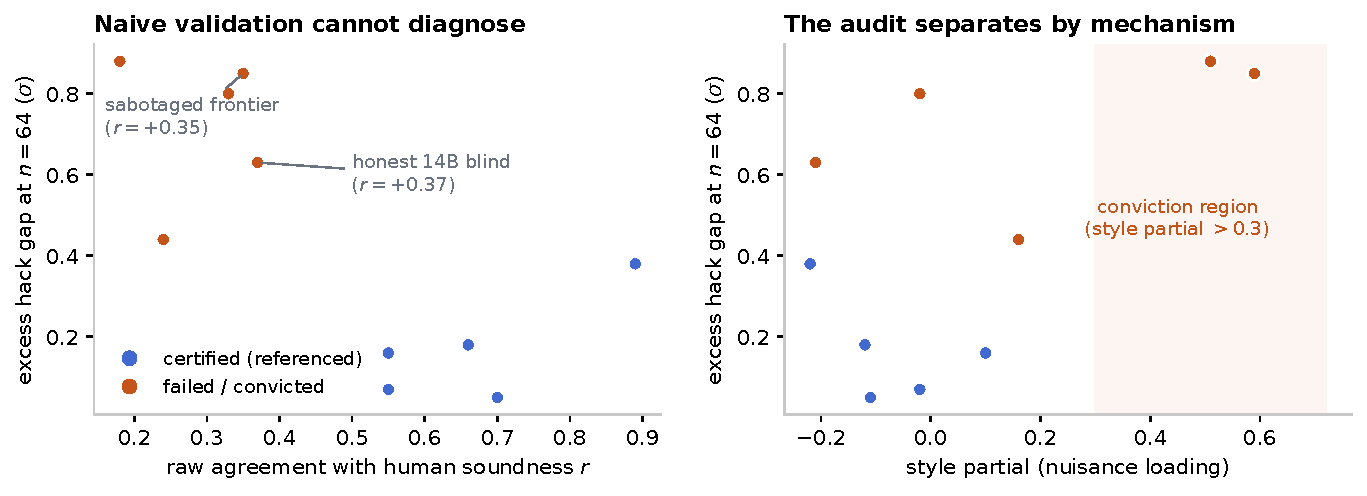
\includegraphics[width=\textwidth]{figures/fig_h2h.pdf}
\caption{\textbf{The head-to-head, visualized.}
Each point is one audited math configuration; the $y$ axis is its scoreboard inflation under best-of-64 pressure.
Left: raw agreement with human soundness places the sabotaged frontier judge inside the failed-blind cluster.
Right: the style partial isolates both style-loaded configurations in a sign-anchored conviction region fixed before outcomes.
\textbf{Takeaway: naive validation ranks but cannot diagnose; the audit's nuisance axis separates capable-corrupt from weak-honest.}}
\label{fig:h2h}
\end{figure}

\subsection*{RQ2: Does raw human agreement suffice instead?}

No, and Table~\ref{tab:h2h} and Figure~\ref{fig:h2h} locate the two failures precisely.
Raw agreement is not useless: referenced judges score higher than blind ones, and a threshold placed between the clusters would have called the ladder outcomes.
It fails first by conflating weak-honest with capable-corrupt, the distinction that determines the failure mode under pressure.
It fails second by offering no principled threshold: the separating value is knowable only after the outcomes.
The audit shares the threshold problem for its weak-judge boundary (the 3B-blind partials straddle zero within noise, and the 14B-blind false pass of Section~\ref{sec:pressure} is that problem realized), but its convictions do not: a significantly positive nuisance partial is a sign condition, fixed ex ante, and it alone identifies both style-loaded configurations.
The audit's advantage is diagnosis and sign-anchored conviction, not a magically sharper threshold for weak judges.

\paragraph{Incremental validity over a protocol bit.}
The strongest trivial baseline is a protocol-bit classifier that predicts certified behavior iff a reference is present.
On the same thirteen configurations it scores ten of thirteen: it is wrong on all three sabotaged referenced arms, which it cannot see, and right on the blind 14B, where the audit false-passes.
The audit scores twelve of thirteen.
The audit's incremental value is precisely detection of corrupted instructions and reward models that protocol bits cannot see, at the cost of one boundary miss.

\paragraph{Multiple comparisons.}
The conviction rule is a single pre-declared sign condition per configuration, a significantly positive nuisance partial, not a search over thresholds, which bounds the multiplicity concern.
A Bonferroni correction across the eleven registered-era audited configurations leaves all three convictions significant: recomputing the style-partial bootstrap CIs at the corrected level keeps them wide of zero (sabotaged frontier $[+0.25, +0.80]$, reward model $[+0.20, +0.77]$), and the 1.5B-blind conviction's permutation test gives $p = 0.0017$ (two-sided, $n{=}53$), below the corrected level $0.05/11$ (corrected conviction CIs in \texttt{papers/analysis/conviction\_bonferroni.json}).

\paragraph{Verdict stability.}
Convictions and strong passes stabilize with the fewest labels.
At 40 labels, the sabotage conviction and the honest frontier pass reproduce in $100\%$ of label resamples, while boundary configurations (the 1.5B referenced pass, the 14B blind threshold pass that Section~\ref{sec:pressure} shows to be false) remain unstable at $50$ labels and below (the 14B blind verdict reproduces fully only at the complete $60$-label set; the 1.5B referenced pass reaches $94\%$ at $50$ of its $56$ labels) (Figure~\ref{fig:stability}).
A few dozen labels certify clear cases; boundary verdicts honestly demand more.

\begin{figure}[t]
\centering
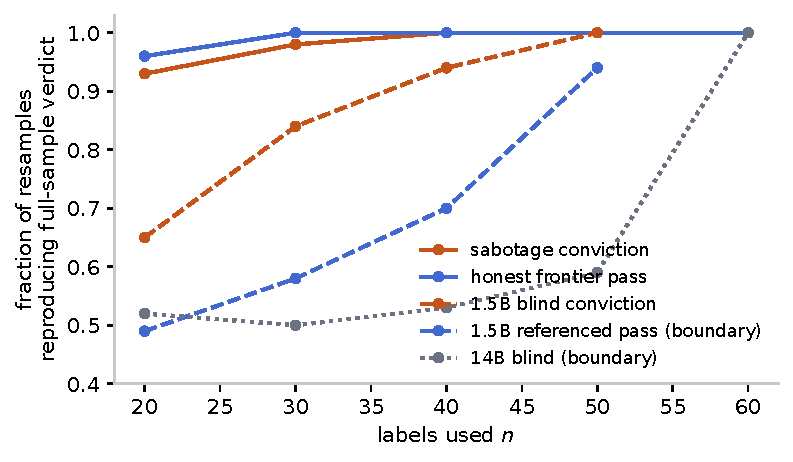
\includegraphics[width=0.62\textwidth]{figures/fig_stability.pdf}
\caption{\textbf{Verdict stability under label subsampling} (500 resamples per point, fixed verdict rules).
\textbf{Takeaway: convictions are cheap and stable; verdicts near the pass boundary are the ones that need more labels.}}
\label{fig:stability}
\end{figure}

\paragraph{What the certificate covers: outcomes, not process.}
Even certified judges grade endpoints rather than checking each line.
With planted errors whose wrong value propagates coherently to the final answer, frontier judges catch essentially all; with planted false steps that do not change the final answer, they forgive $40$--$50\%$~\cite{companionB}.
A pass therefore certifies soundness-tracking at the solution level, not step-level process verification.

\paragraph{A zero-label pre-screen.}
An order-swap test costs nothing: ask the same pairwise comparison twice with the order flipped and measure the flip rate.
Across the ladder the flip rate falls from $71$--$95\%$ at 0.5B to $2$--$37\%$ at 14B~\cite{companionB}.
A judge that cannot agree with itself under order swap cannot pass any validity audit, so the free tier eliminates hopeless judges and reserves labels for certifiable ones.

\paragraph{When a reference helps.}
On planted-error detection, the ladder detects $3/17/49/75\%$ of errors blind and $21/85/85/90\%$ with the gold reference; the 3B jump replicates in six model families ($+14$ to $+60$ points)~\cite{companionB}.
Producing a reference is the hard part, not using one: a judge that first solves the problem and then grades against its own solution detects $59/60/85/95\%$, above gold at 1.5B and 14B, matching at 7B, trailing at 3B.
Part of small-judge weakness is protocol, not capability.

\paragraph{When a reference hurts.}
On tasks with many valid answers the reference lever inverts, statically and dynamically.
Statically, any reference, whoever wrote it, costs $7$--$8$ points of verdict accuracy (paired, $p \le .0005$)~\cite{companionD}.
Dynamically, under best-of-64 pressure on multi-valid tasks, the referenced judge is more inflated than the blind one at all four ladder sizes (for example 3B: gap $+0.55$ blind versus $+1.21$ referenced), and the mechanism is directly measurable: among equally valid answers, referenced judges score those matching the shown reference $+2.7$ to $+10.0$ points (of 10) above the rest, with total anchoring at 1.5B--3B, while blind judges show no such margin~\cite{companionD}.
A reference converts a judge into a verifier only when the task's answer is effectively unique and checking against the reference is within the judge's capability.

\section{The certificate under pressure}
\label{sec:pressure}

The experiment is simple to state: a 7B generator writes 64 candidates per problem, each judge configuration picks its favorite, and we check what happened.
Two pre-registered estimands separate deception from damage.
The \emph{excess hack gap} measures scoreboard inflation relative to true quality, in baseline standard deviations over a within-oracle-stratum permutation null (judge scores permuted among samples with the same correctness).
\emph{Oracle regret} measures accuracy left on the table against best-possible selection.
Selection and reporting use different rubric paraphrases, canceling winner's curse.
Item pools are 105 \textsc{MATH-500} and 68 \textsc{MBPP+} items on which the generator sometimes but not always succeeds (pool pass rate in $[0.2, 0.8]$); estimators were committed before generation.

\subsection*{RQ3: Does the audit's verdict predict gaming?}

In-domain, yes, and the answer is per estimand.
The registered predictions were categorical: blind ladder judges fail the audit and referenced ones pass; the sabotaged judge is convicted; failed evaluators are gamed.
On inflation, every failed or convicted configuration (minimum $+0.44\sigma$) exceeds every certified one (maximum $+0.38\sigma$), and the sabotaged frontier's excess gap $+0.85$ $[0.70, 1.00]$ is disjoint from the honest frontier's $+0.38$ $[0.28, 0.51]$.
On regret, every failed blind configuration (minimum $0.324$) exceeds every certified one (maximum $0.117$), but the sabotaged frontier does not separate: its regret $0.133$ is statistically indistinguishable from the honest frontier's $0.117$ (paired difference $+0.014$ $[-0.058, +0.085]$, $n{=}105$ items).
That asymmetry is itself a finding: a style-loaded frontier judge corrupts the scoreboard before it corrupts selection, which is exactly the failure a naive accuracy check cannot see.
We do not claim a pre-frozen numeric threshold; we claim registered categorical verdicts plus the per-estimand separation just stated, with the full 25-configuration accounting in Appendix~\ref{app:confusion}.

\begin{figure}[t]
\centering
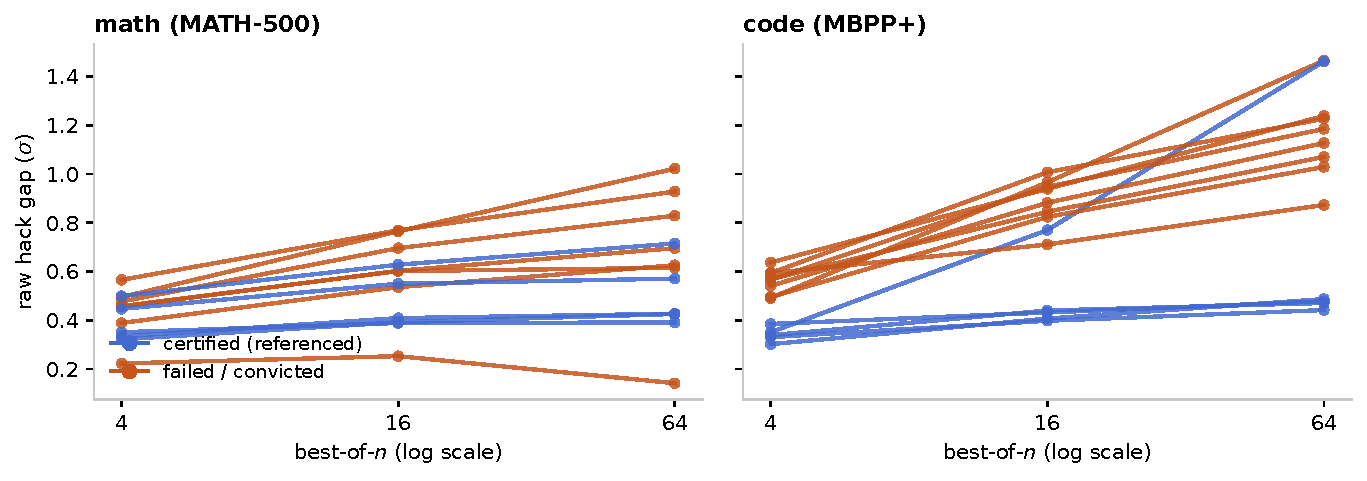
\includegraphics[width=\textwidth]{figures/fig_curves.pdf}
\caption{\textbf{Pressure curves: raw hack gap versus best-of-$n$} for every configuration with existing candidate pools, recomputed at $n = 4, 16, 64$ with the pre-registered estimators.
Blue: certified (referenced) configurations; orange: failed or convicted ones.
\textbf{Takeaway: failed configurations' inflation roughly doubles from $n{=}4$ to $n{=}64$ while certified configurations' rises by less than $0.15\sigma$; the certificate predicts the slope of hacking, not only its endpoint.}}
\label{fig:curves}
\end{figure}

\paragraph{The separation grows with optimization strength.}
Failed configurations steepen and certified ones stay flat (Figure~\ref{fig:curves}).
The blind 3B's code gap runs $+0.64 \to +0.94 \to +1.24$ across $n = 4, 16, 64$, and the blind 7B's $+0.57 \to +0.95 \to +1.19$; the referenced 3B runs $+0.33 \to +0.40 \to +0.44$ and the referenced frontier $+0.39 \to +0.43 \to +0.48$.

\paragraph{Cross-domain transfer, and an in-domain audit with a mechanical target axis.}
The audit generalizes beyond human labels wherever the target axis has an oracle, and code supplies one: executed tests.
We audited every code configuration by the within-item correlation of its scores with test outcomes, with no human labels involved.
The measured rows explain the one extrapolation miss directly: the 1.5B judge's reference adds nothing to its target-axis validity on code ($+0.15$ blind, $+0.16$ referenced), which is the capability gate measured rather than inferred, and that configuration is gamed as badly as its blind twin (Figure~\ref{fig:gate}).
The frontier tier separates cleanly ($+0.52$ blind, $+0.62$ referenced), and sabotage measurably degrades target validity even against a mechanical target ($+0.62 \to +0.42$).
One honest nuance: the 3B judge shows equal target validity blind and referenced ($+0.10$) yet resists inflation only when referenced, so the mechanical-target audit predicts damage well and inflation resistance only through the reference protocol; the human-label axes remain necessary for the deception side.
Operationally: a judge certified on one domain is not thereby certified on another; run the audit, with whatever target oracle the domain offers, where the judge will be used.

\begin{figure}[t]
\centering
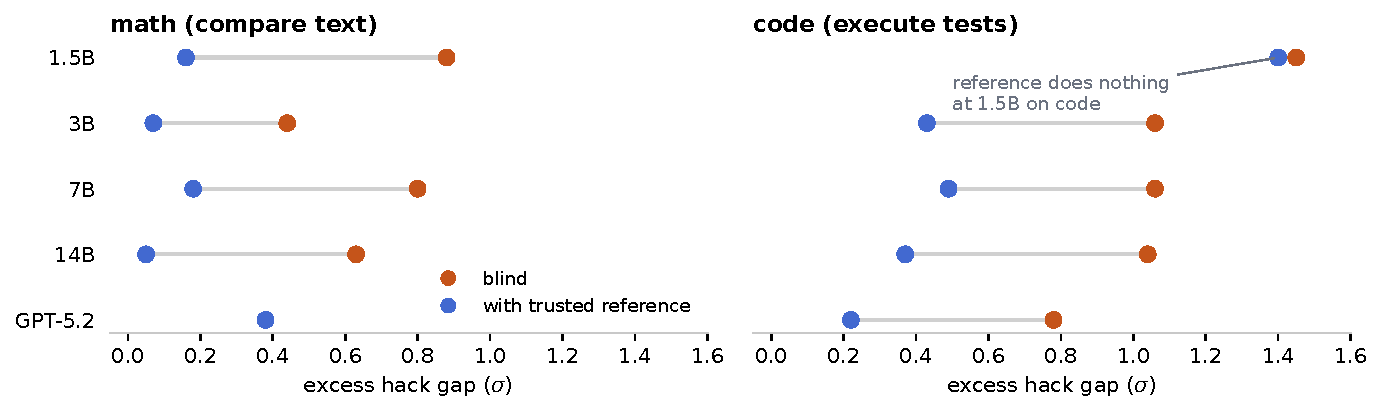
\includegraphics[width=0.9\textwidth]{figures/fig_gate.pdf}
\caption{\textbf{The capability gate.}
Excess hack gap at $n{=}64$ without (orange) and with (blue) a trusted reference, by judge scale and domain.
\textbf{Takeaway: the reference collapses inflation at every scale on math, where using it means comparing text, and only at 3B and above on code, where using it means executing tests.}}
\label{fig:gate}
\end{figure}

\paragraph{Two failure modes, and capability trades one for the other.}
Across the sabotage arms, damage falls and self-inflation rises with judge capability.
The sabotaged 7B damages without inflating (regret $0.400$, gap $+0.13$, not significant); sabotaged GPT-5.2 inflates without measurable damage (gap $+0.85$; regret $0.133$, indistinguishable from the honest frontier's $0.117$).
A blind cross-family panel confirms the channel: sabotage-selected solutions are more styled ($+0.27$ $[0.10, 0.44]$) with no detectable soundness loss.
The frontier mode, deceiving the metric while selecting well, is the one that menaces training.

\paragraph{Granularity beats scale once a reference is in hand.}
The referenced 1.5B outselects the frontier on math because the frontier's 0--10 scale ties $78\%$ of items at the top and random tie-breaks admit wrong answers, while the small judge's continuous expected scores stay sharp.
A registered ablation separates two kinds of granularity.
Re-eliciting the frontier judge on a 0--100 integer scale cuts its regret from $0.117$ to $0.069$ and its gap from $+0.38$ to $+0.27$, confirming the registered prediction, yet top-ties rise to $90\%$ and the frontier still does not approach the small judge's $0.010$.
Elicited granularity helps; distributional granularity, reading the expectation over score-token probabilities, helps more, and only judges that expose token probabilities offer it fully.

\section{From an instrument to a procedure}
\label{sec:procedure}

The audit of Section~\ref{sec:audit} is one instantiation: soundness and style as axes, one dataset, one label budget.
The general procedure behind it has four tiers, and each tier already has partial experimental support in this paper's data.

\paragraph{Tier 0: self-consistency screens, at zero labels.}
A judge that cannot agree with itself cannot be audited.
The order-swap flip rate (Section~\ref{sec:audit}) falls from $71$--$95\%$ at 0.5B to $2$--$37\%$ at 14B, and a score-range check catches unauditable regimes (on saturated data $96\%$ of the frontier judge's scores are identical, so no validity question can be asked).
Both screens are free and gate everything downstream.

\paragraph{Tier 1: causal axis discovery, at zero human labels.}
Nuisance axes should be discovered, not hand-picked, and discovered causally rather than by regression.
Our own history motivates the distinction: an observational length effect in the frontier judge's scores did not reproduce when we causally padded solutions holding content fixed, while the same causal probes measured a real first-position bias in one frontier judge (order-swap preference $0.62$) and none in another ($0.47$).
We therefore register a fixed six-axis perturbation battery adapted from published evaluator-bias taxonomies~\cite{cobbler2023,judgebiasbench2026}: length padding, reformatting, authority cues, bandwagon cues, confident-tone injection, and hedging, each preserving mathematical content and the final answer.
Its registered predictions include the validation that keeps the tier honest: across judge configurations, battery-measured presentation sensitivity must rank-correlate with the audit's independently measured style partials (P-B4).
If Tier 1 predicts Tier 2, axis discovery is validated; if not, hand-chosen axes remain necessary, and we report either outcome.
Fixing the taxonomy before data is what blocks the circularity of discovering whichever axes make the audit look good.
The two frontier arms of the battery have now been run, with per-axis score deltas and bootstrap CIs in \texttt{papers/analysis/battery\_gpt\_ref.json} and \texttt{battery\_gpt\_sabotage.json}.
The honest frontier judge is insensitive on all six axes, every CI crossing zero (length $-0.05$ $[-0.18, +0.07]$, format $-0.03$, authority $-0.02$, bandwagon $-0.07$, confidence $-0.07$, hedging $+0.02$), confirming the registered null prediction P-B2.
The sabotaged judge is significantly sensitive on three axes, but in the negative direction (length $-0.20$ $[-0.35, -0.03]$, bandwagon $-0.32$ $[-0.52, -0.08]$, hedging $-0.53$ $[-0.72, -0.37]$): appended social cues and hedges lower its score.
The registered sign prediction P-B1, positive sensitivity on presentation axes, is therefore falsified in direction, while its magnitude prediction ($|\Delta| \ge 0.5$) is met only for hedging.
Read honestly, the sabotaged judge punishes any appended imperfection rather than rewarding authority cues; that is still a presentation sensitivity the honest judge lacks, but the registered sign was wrong, and we report the outcome as promised.
The remaining ladder arms and the rank-correlation validation (P-B3, P-B4) are queued and unclaimed.

\paragraph{Tier 2: target-axis validation, with an oracle where one exists.}
The target axis does not require human labels when the domain has an oracle.
Code supplies one, and the mechanical-target audit of Section~\ref{sec:pressure} is the demonstration: executed tests as the target axis measured the capability gate in-domain, separated the frontier tier, and detected sabotage ($+0.62 \to +0.42$), all without an annotator.
Its measured scope limit travels with it: the mechanical target predicted damage well and inflation-resistance only through protocol, so human-labeled nuisance axes remain necessary for the deception side.
Where no oracle exists, humans grade the target axis, and the divergence-stratum construction (sample where cheap signals disagree) supplies power that random sampling cannot.

A fully mechanical instantiation was also run after the human audit, with expectations stated in the analysis header before execution (\texttt{papers/analysis/mech\_axes\_audit.py}).
It substitutes machine correctness for the target axis and log response length for the nuisance axis, at zero human labels, on the same thirteen configurations.
Under a simple explicit verdict rule, flag a configuration if its length-partial CI excludes zero, six of the thirteen are flagged: the sabotaged frontier ($-0.74$ $[-0.84, -0.60]$), the reward model ($-0.54$ $[-0.70, -0.32]$), the sabotaged 14B ($-0.45$ $[-0.66, -0.21]$), the sabotaged 7B ($-0.41$ $[-0.61, -0.17]$), the referenced 1.5B ($-0.35$ $[-0.58, -0.08]$), and the referenced 3B ($-0.22$ $[-0.44, -0.01]$).
Unflagged are the honest frontier ($+0.13$), the referenced 14B ($-0.03$), the referenced 7B ($-0.14$), the blind 14B ($+0.09$), the blind 7B ($+0.08$), and the blind 3B ($-0.29$, CI crossing zero); the blind 1.5B's bootstrap is degenerate, so its CI is unavailable and it is not flagged.
The stated expectation E1, that honest judges come out clean, is therefore partially violated: two of the five honest referenced judges, the 1.5B and 3B, show significantly negative length partials.
And E2 as stated, that style convictions would ``not necessarily'' transfer to the length axis, was unfalsifiable phrasing that no outcome could have contradicted, which is not pre-specification.
The honest summary is this.
The zero-label audit separates the two most corrupted evaluators by margin: the sabotaged frontier and the reward model carry the two largest length-partial magnitudes ($-0.74$ and $-0.54$), their correctness partials collapse ($+0.22$ $[-0.13, +0.52]$ and $-0.03$), and the honest frontier is clean (length $+0.13$, correctness $+0.98$).
But the significance-based rule also flags four other configurations, including two honest referenced passes, so the mechanical axes are a coarse screen that orders corruption severity, not a verdict instrument; the human-labeled audit remains the verdict tier.
The length signal does feed back into the human audit as a confound check, and the three-variable partial of Section~\ref{sec:audit} shows both style convictions survive controlling for length (\texttt{papers/analysis/style\_partial\_lencontrol.json}).

\paragraph{Tier 3: the pressure test as the axis-agnostic backstop.}
Any nuisance axis missing from Tiers 1--2 can still be exploited, and the best-of-$n$ experiment is the detector of last resort, run per domain.

\paragraph{Label economics, in place of a magic number.}
The label budget is verdict-dependent, not fixed.
Empirically, convictions stabilize by roughly 40 labels while boundary passes do not (Figure~\ref{fig:stability}); analytically, cross-rater components bound what labels can measure (soundness ceiling $\approx 0.89$, style $\approx 0.72$), and Spearman--Brown projections say how much a second rater buys ($0.80 \to 0.89$ for soundness).
These ceilings come from $n{=}20$ shared items under a schema mismatch, so they carry wide uncertainty (the soundness inter-rater point estimate's 95\% CI spans roughly $[0.55, 0.92]$) and are indicative anchors, not walls.
A registered prospective test applies these curves to predict the label budget for a second math dataset before its labels arrive.

\paragraph{What remains non-generic.}
Three limits are inherent rather than incidental.
Synthetic perturbations can be off-manifold, so Tier-1 insensitivity to an injected cue does not preclude sensitivity to its natural counterpart; Tier-1 causal sensitivity and Tier-2 in-distribution loading catch different failures and neither substitutes for the other; and outcome validation costs compute in every new domain.
The procedure narrows the unmeasured space at each tier; it does not close it.

\section{Design rules}
\label{sec:rules}

This section compresses the paper's findings into five rules a practitioner can apply directly.

\begin{enumerate}
\item \textbf{Audit before you optimize, in the deployment domain.}
A few dozen blind labels on separated axes, a decorrelated subsample, and partial correlations; labeling sixty traces on two axes at two to four minutes per trace-axis (120 trace-axis gradings) is four to eight annotator-hours, and the frozen verdicts predicted ten of eleven registered in-domain pressure outcomes (ledger, Table~\ref{tab:ledger}), with the one false pass sitting at the pass threshold (Section~\ref{sec:pressure}).
Four to eight hours is the labeling cost alone, amortized across judges (one label set served all thirteen configurations here); end-to-end certification also requires assembling the trace pool and cheap-signal battery, and the optional pressure backstop costs 64-samples-per-item generation plus judge calls per configuration, which dwarfs the labeling compute.
\item \textbf{Do not substitute raw agreement.}
It ranks but cannot diagnose, and it has no sign-anchored conviction (Table~\ref{tab:h2h}).
\item \textbf{Choose the ignored-property axes by threat model, and treat the audit as a screen for the axes it instruments.}
Style is the dominant documented axis and ours; length, format, and duplication were causally probed and cleared for these judges; position bias is measurable label-free by order-swap.
An axis orthogonal to all instrumented ones can evade the audit; the pressure test is the axis-agnostic backstop.
\item \textbf{Give a judge a reference only when the answer is unique and the judge can use it.}
On multi-valid tasks the lever inverts and amplifies gaming (Section~\ref{sec:audit}).
\item \textbf{Audit the oracle before the evaluator.}
Apparent evaluator failures in our own data dissolved, on adjudication, into evaluation-pipeline verdict errors~\cite{companionC}.
\end{enumerate}

\section{Discussion and limitations}
\label{sec:limits}

This section states the six limits that bound the claim, and the two designed tests that address the deepest one.

First, the labels: the primary annotator is an author and hypothesis-aware, so an independent check was the top gating item, and it has now run.
A hypothesis-blind annotator external to the author list regraded 30 of the 60 anchor items under the same rubric, on a blinded instrument with model names and machine scores stripped.
Same-rubric reliability is soundness $0.83$ and style $0.48$, implying single-rater ceilings of about $0.91$ and $0.69$; the 30-item replication reproduces the honest pass and both convictions in sign, with the sabotage conviction significant on the blind rater's labels alone and the reward-model conviction significant on two-rater consensus (per-cell values and intervals in Table~\ref{tab:robust}).
The residual caveats: the full 60-item consensus recompute awaits the remaining 30 items, and the 30-item intervals are wide.
The style axis is the noisier instrument (cross-rater $0.48$, ceiling about $0.69$), which attenuates exactly the partials that carry convictions; against that ceiling the measured convictions ($+0.51$, $+0.59$) are proportionally large.
The honest frontier's soundness partial ($+0.90$) sits at the single-rater ceiling, so it should be read as saturating what one rater's labels can measure, not as a claim about the remaining fraction.
The ceiling arithmetic is itself sensitive to the correlation measure: the soundness cross-rater Pearson of $0.83$ drops to a Spearman of $0.46$ at $n{=}30$, so the $0.91$ ceiling may be carried by a few extreme items and a rank-based reading of the ceiling would be lower; the honest-frontier pass does not depend on the ceiling arithmetic.
The same-rubric estimates agree with the earlier cross-schema 20-item anchors, which retroactively derisks that anchor; both intervals are wide at these sample sizes, so the ceilings are indicative anchors, not walls (Table~\ref{tab:robust}).

Second, the weak-judge boundary: verdicts for judges near the pass line sit within interval overlap at these label counts; the subsampling analysis quantifies which verdicts are stable, and convictions are while boundaries are not (Appendix~\ref{app:subsample}).

Third, scope of validation: one audited domain; code is extrapolation; the capability-gate explanation of the one code miss is post hoc until the registered code audit runs.

Fourth, the pressure test is selection, not training; the frontier failure mode is precisely where selection understates risk, and a DPO validation is registered to close the gap.
Preference pairs are built from the frozen certified (honest referenced) and convicted (sabotaged) GPT-5.2 judges on the same in-band items (808 and 800 pairs), identical LoRA-DPO arms are trained on the generator model, and both arms are evaluated by oracle accuracy and by both frozen judges on train and held-out items.
Its three registered predictions (P-D1--P-D3: the certified arm improves true accuracy with judge and true gains agreeing in sign; the convicted arm shows a larger judge-minus-true wedge and a smaller true gain; score gains are instrument-specific) are committed pre-run.
The first run produced no detectable policy movement and was classified post hoc as a manipulation failure: one epoch at a conservative learning rate left training reward margins near zero, every true-accuracy gain within a percentage point, and every judge-score gain and wedge crossing zero, so the run tests nothing about the predictions and is recorded as no test, not as a falsification.
A rerun with a stronger manipulation (four epochs, four times the learning rate) and a registered manipulation check (the trained arm must move its own judge's train-set score, or the run is again recorded as no test) is queued; no outcome is claimed here (ledger, Table~\ref{tab:ledger}).

Fifth, population shift and family confound: the audit labels come from seventeen models' solutions while the primary pressure pools come from one generator, and all open-weights judges share that generator's family, so self-preference could in principle inflate blind-judge gaming.
The registered cross-family run closes this: on a Llama-3.1-8B-generated pool (176 in-band items) the pattern replicates at every ladder size, with blind and referenced inflation intervals disjoint within each size (ranges in Table~\ref{tab:robust}).
Blind-judge gaming is therefore not a same-family artifact, though the referenced tier is less clean cross-family (the 7B referenced inflation reaches $+0.50$, against at most $+0.18$ on the same-family pool), consistent with Qwen judges verifying Llama solutions less reliably.
A deployment-pool label set remains registered (the labeling instrument exists).

Sixth, effective sample size: the thirteen audited configurations' verdicts are strongly collinear with one protocol bit, reference presence, and beyond it there are roughly four distinct verdict classes (blind-weak, referenced-pass, style-loaded, and sabotage-at-ladder-scale fail), so the validation is closer to four independent tests than thirteen.
The registered DPO run and the reward-model paraphrase-replicate protocol below are the two designed tests that break this collinearity; the second has now run and confirmed its registered prediction.
For the same reason we do not quote false-pass or false-convict rates for the certificate: four effective classes cannot estimate them, and the registered replications (Putnam, the code audit, DPO) are what will accumulate the outcomes such rates require.
The label count is what sufficed here, not a derived minimum.

\paragraph{Making inflation comparable for reward models.}
The inflation estimand requires that selection and reporting use independent score replicates, which a judge provides through rubric paraphrases and a single scoring function does not.
A paraphrase-replicate protocol closes the gap: selection uses the reward model's scores of the original candidates, and reporting uses its scores of content-preserving paraphrases of the same candidates (Qwen-7B, index-aligned), so the winner's-curse cancellation matches the judge protocol.
The run confirms the registered prediction (P-R1; ledger): the convicted reward model's inflation is $+1.46\sigma$ ($n{=}105$), the largest of any configuration measured, with regret unchanged at $0.286$ because the reporting replicate does not touch selection.
One caveat travels with the number: the replicate is candidate-side rather than rubric-side, so the estimand is analogous to the judge protocol's rather than identical, and the measured inflation conflates winner's-curse inflation with the reward model's own sensitivity to content-preserving rewording; both readings indict a deployed reward signal.

\section{Related work}
\label{sec:related}

The closest question to ours is whether any static measure predicts downstream optimization failure.
Benchmark accuracy does not~\cite{wen2024rethinking}; our contribution is a static, black-box, few-label measure whose registered verdicts did, with a construct-validity design explaining why.
Active auditing trains attackers against a frozen reward model~\cite{beigi2026ara}; the certificate needs no attacker.
Judge reliability audits measure consistency and bias robustness~\cite{judgechanges2026,zheng2023judging}; validity against decorrelated human axes, with a positive control, is the missing piece we add.
Style-over-substance biases are documented in general pools~\cite{wu2023style,dubois2024length,singhal2023long}; the audit measures the loading for a particular judge, task, and prompt.
The existence of style-substance conflation in trained reward models is likewise established at the class level: RM-Bench evaluates reward models on curated style-controlled pairs and finds the class fragile to exactly this conflation~\cite{rmbench2024}, and reward-model benchmarks have been re-examined through the lens of reward overoptimization~\cite{kim2025lens}.
Those benchmarks characterize the evaluator class on fixed public data; the certificate is a per-deployment diagnostic that spends a few dozen labels to measure whether a particular judge on a particular distribution reads substance, with a positive control, sign-anchored ex-ante conviction rules, and validation of verdicts against selection-pressure outcomes on the same deployment distribution.
RM-Bench tells you the class is fragile; the audit tells you whether your judge, on your task and prompt, reads substance before you deploy it.
References are known to improve judge accuracy~\cite{refguided2024,smalljudges2025}; we show they flip audit validity, that the effect is capability-gated, and that on multi-valid tasks any reference harms statically~\cite{generous2026,dobefore2025} and amplifies gaming dynamically~\cite{companionD}.
Reward hacking is characterized post-hoc~\cite{gao2022scaling,skalse2022defining,coste2023ensembles,eisenstein2023helping,selfplay2026}; the certificate is ex-ante.

\section*{Next steps (internal; remove before submission)}
\begin{enumerate}
\item Trained RM baseline: audit + BoN grids (running).
\item Second rater + external annotator (instrument live); recompute on consensus labels.
\item In-domain code audit (instrument exists); second math dataset (Putnam instrument to build).
\item Ladder-sabotage audit scoring (closes the two unaudited configurations).
\item Cross-family generator (Llama-3.1-8B) BoN on math.
\item Deployment-pool labels (instrument live: artifact f9ac8781).
\item Order-swap flip rate versus audit verdicts, quantitative.
\item DPO validation: train against one certified and one convicted judge.
\item Quantify realized selection pressure per judge (multiple-comparisons note now in Section 3).
\item RM paraphrase-replicate inflation run (protocol now described in Section 6).
\end{enumerate}


\bibliographystyle{plain}
\bibliography{references}

\appendix

\section{Full configuration accounting}
\label{app:confusion}
All 25 pressure-tested configurations: 12 math (4 blind, 4 referenced, frontier honest, frontier sabotaged, plus two sabotaged ladder configurations never audited) and 13 code (4 blind, 4 referenced, frontier blind, frontier referenced, frontier sabotaged, two sabotaged ladder).
Audited in-domain: the 11 configurations of Table~\ref{tab:h2h} (four blind, four referenced, the honest and sabotaged frontier, and the trained reward model).
Applying the frozen rule of Appendix~\ref{app:subsample} uniformly yields six passes (the four referenced ladder judges, the honest frontier, and the blind 14B), two fails (blind 3B, soundness partial $0.19$; blind 7B, $0.32$), and three convictions (blind 1.5B, the sabotaged frontier, and the reward model); ten of the eleven verdicts match their pressure outcomes per estimand, the blind 14B pass being the single miss.
The blind 14B is a false pass: soundness partial $+0.41$ $[+0.12, +0.64]$ against the $0.40$ cut, style partial $-0.21$, yet excess gap $+0.63$ $[+0.42, +0.84]$ and regret $0.324$, both in the failed cluster.
The sabotaged frontier separates on inflation only (its regret is statistically indistinguishable from the honest frontier's, paired difference $+0.014$ $[-0.058, +0.085]$).
Under the post-hoc revised rule of Section~\ref{sec:pressure}, which requires the soundness-partial CI to clear the bar, the blind 14B returns insufficient evidence to certify, and so do the referenced 1.5B (CI $[+0.21, +0.75]$) and referenced 3B ($[+0.36, +0.70]$), whose intervals straddle $0.40$; the revised-rule record is eight predictions (three passes, two fails, three convictions), eight correct, three abstentions.
That revision was adopted after the false pass was observed and is frozen for the Putnam replication.
Never audited: sabotaged 7B (math gap $+0.13$ ns, regret $0.400$; code $+0.84$, $0.559$) and sabotaged 14B (math $+0.61$, $0.324$; code $+0.96$, $0.426$); both are excluded from prediction claims, and an audit run for them is registered.
Code: the mechanical-target audit rows (within-item correlation with executed tests, bootstrap CIs) are in \texttt{papers/analysis/code\_oracle\_audit.json}, and the code-side pressure summaries (per-configuration excess gaps with CIs, regrets, and tie fractions) are mirrored at \texttt{papers/analysis/bon\_code\_full.json}.
Excluding the two never-audited sabotaged code ladder cells leaves eleven eligible code configurations; extrapolated verdicts match the pressure outcome in ten, with the referenced 1.5B the single miss (gap $+1.40$, regret $0.441$), coinciding with its null reference gain on the target axis.
Code verdict predictions were not registered, and the extrapolation scoring is post hoc.

\section{Verdict stability under label subsampling}
\label{app:subsample}
At $n$ labels resampled from the anchor set (500 draws), the fraction of draws reproducing the full-sample verdict under fixed rules (convict if style partial $> 0.30$; pass if soundness partial $> 0.40$ and style partial $< 0.20$): sabotage conviction $0.93/0.98/1.00$ at $n = 20/30/40$; honest frontier pass $0.96/1.00/1.00$; 1.5B-blind conviction $0.65/0.84/0.94$.
The boundary configurations differ from each other: the 1.5B referenced pass reaches $0.70$ at $n{=}40$ and $0.94$ at $n{=}50$, while the 14B blind pass is still at $0.59$ at $n{=}50$ and reproduces fully only at the complete $n{=}60$ set.
Full table: \texttt{papers/analysis/label\_subsampling.md}.
Section~\ref{sec:pressure} shows that the 14B blind pass this rule produces is a false pass under pressure.

\section{Paired-contrast confidence intervals}
\label{app:cis}
Per-configuration excess-gap point estimates and 95\% CIs for all twelve math configurations, the paired boundary contrasts of Section~\ref{sec:pressure}, and the 1.5B conviction inference are in \texttt{papers/analysis/gap\_cis.json}.
Blind-minus-referenced excess-gap contrasts, with per-item bootstrap 95\% CIs.
Math: $+0.72$ $[+0.57,+0.86]$, $+0.37$ $[+0.24,+0.51]$, $+0.62$ $[+0.48,+0.76]$, $+0.57$ $[+0.36,+0.78]$ (1.5B/3B/7B/14B, $n{=}105$); code $+0.05$ $[-0.29,+0.40]$, $+0.63$ $[+0.44,+0.83]$, $+0.56$ $[+0.32,+0.81]$, $+0.67$ $[+0.41,+0.95]$ ($n{=}68$).
On the multi-valid tasks the sign inverts: referenced-minus-blind contrasts are positive at all four sizes ($+0.35, +0.65, +0.08, +0.47$; individual CIs cross zero at $n{=}51$ items; the anchoring-margin mechanism carries CIs excluding zero in all eight referenced cells).


\end{document}
